%% Preamble
  \documentclass{homework}

  \hwTitle{Assignment\ \#6 - Magnetostatics} % Assignment title
  \hwDueDate{Friday,\ June\ 14,\ 2013} %  Due date
  \hwClass{Physics\ 441} % Course/class
  % \hwInstructor{Manuel Berrondo} % Teacher/lecturer
  \hwAuthor{Spencer Lyon} % Your name

  \usepackage{setspace}

  %% Added by Spencer for source code highlighting
  \usepackage{listings}
  \usepackage{color}

  \definecolor{dkgreen}{rgb}{0,0.6,0}
  \definecolor{gray}{rgb}{0.5,0.5,0.5}
  \definecolor{mauve}{rgb}{0.58,0,0.82}

  \lstset{frame=tb,
    language=Python,
    aboveskip=3mm,
    belowskip=3mm,
    showstringspaces=false,
    columns=flexible,
    basicstyle={\small\ttfamily},
    numbers=left,
    stepnumber=5,
    numberstyle=\tiny\color{gray},
    keywordstyle=\color{blue},
    commentstyle=\color{dkgreen},
    stringstyle=\color{mauve},
    breaklines=true,
    breakatwhitespace=true
    tabsize=4
  }

  % Declares the font
  \usepackage{calligra}
  \DeclareMathAlphabet{\mathcalligra}{T1}{calligra}{m}{n}
  \DeclareFontShape{T1}{calligra}{m}{n}{<->s*[2.2]callig15}{}

  % Makes '\sr' make a script r
  \newcommand{\sr}{\ensuremath{\mathcalligra{r}}}

% New commands I use a lot
  \newcommand\ve{\varepsilon}
  \newcommand{\bs}[1]{\ensuremath{\boldsymbol{#1}}}
  \newcommand{\bhat}[1]{\ensuremath{\boldsymbol{\hat{#1}}}}
  \newcommand{\cross}[2]{\ensuremath{\boldsymbol{#1} \times \boldsymbol{#2}}}
  \newcommand{\curl}[1]{\ensuremath{\cross{\nabla}{\bs{#1}}}}
  \newcommand{\diver}[1]{\ensuremath{\nabla \times \bs{#1}}}

  % partial derivative as a fraction
  \newcommand{\fracpd}[2]{
    \ensuremath{\frac{\partial #1}{\partial #2}}
  }

  % partial derivative as a fraction with evaluation bounds
  \newcommand{\fracpdb}[3]{
    \ensuremath{\left. \frac{\partial #1}{\partial #2} \right|_{#3}}
  }

  % Just a vector in xhat yhat zhat
   \newcommand{\xyzvec}[3]{
   \ensuremath{
      (#1) \bhat{x} + (#2) \bhat{y} + (#3) \bhat{z}
   }
   }

  % fraction with parenthesis around it
  \newcommand{\pfrac}[2]{
    \ensuremath{ \left( \frac{#1}{#2} \right)}
  }

% Problems in this assignment
% 5.2 -> 5.2
% 5.4 -> 5.4
% 5.8 -> 5.8
% 5.10 -> 5.10
% 5.15 -> 5.14
% 5.23 -> 5.22
% 5.25 -> 5.24
% 5.34 -> 5.33


\begin{document}

\maketitle

\begin{homeworkProblem}[Problem 5.2]

  Find and sketch the trajectory of the particle in Example 5.2, if it starts at the origin with three different velocities:

  \begin{enumerate}
    \item  $\bs{v}(0) = (E/B) \bhat{y}$
    \item  $\bs{v}(0) = (E/2B) \bhat{y}$
    \item  $\bs{v}(0) = (E/B) (\bhat{y}  +\bhat{z}$
  \end{enumerate}

  \vspace{.2in}

  \problemAnswer{ % Answer

    For this problem we have a magnetic field (\bs{B}) in the \bhat{x} direction and an electric field (\bs{E}) in the \bhat{z} direction. We will begin at the general solution found in equation 5.6: $$ y(t) = C_1 \cos(\omega t) +  C_2 \sin(\omega t) + \frac{E}{B} t +  C_3 \quad z(t) =  C_2 \cos(\omega t) -  C_1 \sin(\omega t) + C_4$$. In each case we just need to apply initial conditions to determine the constants $C_1 - C_4$ (At the beginning of each part I will list the initial conditions for time $t=0$, without writing "$(0)$" every time. Also note that I just plug $t=0$ into the trig functions directly and don't write it out to save time).

    Below I will write the derivatives of this general solution with respect to $y$ and $z$, because I will need it.

    $$ \dot{y}(t) = \frac{E}{B}-c_1 \omega  \sin (t \omega )+c_2 \omega  \cos (t \omega ) \quad \dot{z}(t) = c_1 (-\omega ) \cos (t \omega )-c_2 \omega  \sin (t \omega )$$

    \begin{enumerate}
      \item $x=y=z=\dot{x}=\dot{z} = 0$ and $\dot{y} = E/B$ now we will plug the 4 non-trivial boundary conditions in:
        \begin{enumerate}
          \item $\dot{y}(0) = E/B = \frac{E}{B}+c_2 \omega \rightarrow c_2 = 0$
          \item $\dot{z}(0) = 0 = c_1 (-\omega ) \rightarrow c_1=0 $
          \item $y(0) = 0 = C_1 + C_3 $, we already know that $c_1 = 0$, so this tells us that $c_3 = 0$
          \item $z(0) = 0 = C_2 + C_4 = 0$, we already know that $c_2 = 0$, so this tells us that $c_4 = 0$
        \end{enumerate}

      We just learned that all constants are zero, so there is no net force and the particle continues with its velocity. In other words $y(t) = v_{y, 0} t = \frac{E}{B} t$
      \item $x=y=z=\dot{x}=\dot{z} = 0$ and $\dot{y} = E/2B$ now we will plug the 4 non-trivial boundary conditions in:
        \begin{enumerate}
          \item $\dot{y}(0) = E/2B = \frac{E}{2}+c_2 \omega \rightarrow c_2 = -\frac{E}{2B} \omega$
          \item $\dot{z}(0) = 0 = c_1 (-\omega ) \rightarrow c_1=0 $
          \item $y(0) = 0 = C_1 + C_3 $, we already know that $c_1 = 0$, so this tells us that $c_3 = 0$
          \item $z(0) = 0 = C_2 + C_4 = 0$, we already know that $c_2 = -\frac{E}{2B} \omega$, so this tells us that $c_4 = \frac{E}{2B} \omega$
        \end{enumerate}

        We now plug these constants in to get the answer:

        $$y(t) = \frac{E (2 t-\omega  \sin (t \omega ))}{2 B} \quad z(t) = -\frac{E \omega  (\cos (t \omega )+1)}{2 B}$$
      \item $x=y=z=\dot{x} = 0$ and $\dot{y}= \dot{z}= E/B$ now we will plug the 4 non-trivial boundary conditions in:
        \begin{enumerate}
          \item $\dot{y}(0) = E/B = \frac{E}{B}+c_2 \omega \rightarrow c_2 = 0$
          \item $\dot{z}(0) = E/2b = c_1 (-\omega ) \rightarrow c_1= - \frac{E}{\omega B} $
          \item $y(0) = 0 = C_1 + C_3 $, we already know that $c_1 = - \frac{E}{\omega B}$, so this tells us that $c_3 =  \frac{E}{\omega B}$
          \item $z(0) = 0 = C_2 + C_4 = 0$, we already know that $c_2 = 0$, so this tells us that $c_4 = 0$
        \end{enumerate}

        We now plug those in to get the expressions for the trajectory:

        $$ y(t) = \frac{E (t \omega -\cos (t \omega )+1)}{B \omega } \quad z(t)= \frac{E \sin (t \omega )}{B \omega }$$
    \end{enumerate}

    For the sketches see Figure~\ref{fig:p4.2_sketches}

    \qed

  }

    \begin{figure}[!h]
    \begin{centering}
    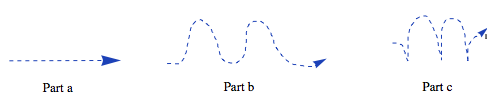
\includegraphics[width=4.5in, height=1.3in]{sketchesP4_2.png}
    \caption{The trajectory of the particles described in problem 4.2}
    \label{fig:p4.2_sketches}
    \end{centering}
  \end{figure}
\end{homeworkProblem}

\begin{homeworkProblem}[Problem 5.4]

  Suppose that the magnetic field in some region has the form $$\bs{B} = kz \bhat{x}$$ (where $k$ is a constant). FInd the force on a square loop (side $a$), lying in the $yz$ plane and centered at the origin, if it carries a current $I$, flowing counter clockwise, when you look down the $x$ axis.  % WORST RUN-ON EVER!

  \vspace{.2in}

  \problemAnswer{ % Answer

    Our problem is very similar to equation Example 5.3 where they say that $F_{\text{mag}} = I B a$.  We will need to apply this to each of the 4 sides of the square:

    \begin{enumerate}
      \item Bottom: $Ia B = - I k a^2 / 2$
      \item Top : $Ia B = I k a^2 / 2$
      \item Left and Right cancel each other.
    \end{enumerate}

    Looking at those pieces we see that the negative on the expression for the bottom tells us that it points in the \bhat{z} direction, where as the positive on the expression for the top also tells us that is points in the \bhat{z} direction. So, the final expression is $$\bs{F} = \text{bottom} + \text{top} = - (- I k a^2 / 2) + I k a^2 / 2 = I k a^2$$

    \qed

  }
\end{homeworkProblem}

\begin{homeworkProblem}[Problem 5.8]

  \begin{enumerate}
    \item Find the magnetic field at the center of a squrqe loop, which carries a steady current $I$. Let $R$ be the distance from center to side (see Figure 5.22)
    \item Find the field at the center of a regular $n$-sided polygon, carrying a steady current $I$. Again, let $R$ bet he distance from the center to any side.
    \item Check that your formula reduces to the field at the center of a circular loop, in the limit $n \rightarrow \infty$
  \end{enumerate}

  \vspace{.2in}

  \problemAnswer{ % Answer

    We will use the form of the Biot-Savart Law (general form Equation 5.34) for cases where $\bs{I}$ is a constant $I$. This is given in equation 5.37: $$ B = \frac{\mu_0 I}{4 \pi s} (\sin \theta_2 - \sin \theta_1)$$

    \begin{enumerate}
      \item In this case we can say that $s= R$, $\theta_1 = - \pi /4$, and $\theta_1 = \pi /4 $ for each side. Plugging those in we get $\frac{I \mu _0}{2 \sqrt{2} \pi  R}$, but we need to do the same for all 4 sides. If we multiply our answer by 4 we get the right answer and we end up with: $$\frac{\sqrt{2} i \mu _0}{\pi  R}$$
      \item In this case we can say that $s= R$, $\theta_1 = - \pi /n$, and $\theta_1 = \pi /n$ for all n sides. We plug in an multiply by $n$ to get the answer: $$\frac{I \mu _0 n \sin \left(\frac{\pi }{n}\right)}{2 \pi  R} $$
      \item As we saw, our angle has a $1/n$ relation to the number of sides. So as $n \rightarrow \infty: \theta -> 0$  and $\sin \theta \rightarrow \theta$. In that case we en up getting. $$B = \frac{n \mu_0 I}{2 \pi R} \pfrac{\pi}{R} = \frac{\mu_0 I}{2 R}$$This is what we want.
    \end{enumerate}

    \qed

  }
\end{homeworkProblem}

\begin{homeworkProblem}[Problem 5.10]

  \begin{enumerate}
    \item Find the force on a square loop placed as shown in Figure 5.24(a), near an infinite straight wire. Both the loop and the wire carry a steady current $I$.
    \item Find the force on the triangular loop in Figure 5.24(b).
  \end{enumerate}

  \vspace{.2in}

  \problemAnswer{ % Answer

    \begin{enumerate}
      \item We will break this problem into the 4 sides of the square and use equation 5.38 to find the magnetic field on each side: $$B = \frac{\mu_0 I}{2 \pi s}$$ We will also use the equation from page 218 to go from the magnetic field to the force: $$F = B I a$$
        \begin{enumerate}
          \item Left and Right: By symmetry these cancel, so we will not worry about them here
          \item Top: We apply the equations with $s = (a + s)$ and get $B = \frac{\mu_0 I}{2 \pi (s + a)}  \rightarrow F = \frac{\mu_0 I^2 a}{2 \pi (s + a)} $
          \item Bottom: We apply the equations with $s = s$ and get $B = \frac{\mu_0 I}{2 \pi s}  \rightarrow F = \frac{\mu_0 I^2 a}{2 \pi s} $
        \end{enumerate}
        In all cases the force points in towards the venter of the circle and we sum to get the net force (note that it goes through the of the square)

        $$F = F_{\text{top}} + F_{\text{bottom}} =  \frac{\mu_0 I^2 a}{2 \pi s}  + \frac{\mu_0 I^2 a}{2 \pi (s + a)}  = \frac{\mu_0 I^2 a^2}{2 \pi s (s + a)}$$

      \item We will break this problem into the three legs of the triangle and use equation 5.38 from above together with equation 5.17 $$\bs{F} = I \int (d \bs{l} \times \bs{B}) $$
        \begin{enumerate}
          \item Bottom: Same as above: $F =  \frac{\mu_0 I^2 a}{2 \pi s} $
          \item Left and Right: We can, by symmetry, say these are equal, but they point in different directions so they don't cancel this time. We will just compute it for one of them and then include it twice when we sum for the total force. WE can say that $\bs{B} = \frac{\mu_0 I}{2 \pi y} \bhat{z}$. We then use equation 5.17 and get an expression for $ \bs{F}$  (Note that when it comes time to actually do the integral I let the computer do it for me).

          \begin{align*}
            \bs{F} &= I \int (d \bs{l} \times \bs{B}) \\
              &= I \int (dx \bhat{x} + dy \bhat{y} + dz \bhat{z}) \times \pfrac{\mu_0 I}{2 \pi y } \bhat{z} \\
              &= \int \frac{\mu_0 I^2}{2 \pi y} (dy \bhat{x} - dx \bhat{y})\\
              &= - \frac{\mu_0 I^2}{ 2 \pi} \left( \int \frac{1}{y} dx + \int 0 dy\right)\\
              &= - \frac{\mu_0 I^2}{ 2 \pi} \int_{2 / \sqrt{3}}^{(s / \sqrt{3} + a / 2)} \frac{1}{\sqrt{3} x} dx \\
              &= - \frac{\mu_0 I^2}{2 \sqrt{3} \pi} \ln \pfrac{s / \sqrt{3} + a/2}{s / \sqrt{3}}
          \end{align*}
        \end{enumerate}

      We now just sum them up to get the final expression for the force on the triangle (note, again I let the computer simplify the algebra):

      $$F = \frac{\mu_0 I^2}{2 \pi} \left(1 - \frac{2}{3}\ln \pfrac{s / \sqrt{3} + a/2}{s / \sqrt{3}}  \right) $$

    \end{enumerate}

    \qed

  }
\end{homeworkProblem}

\begin{homeworkProblem}[Problem 5.15]

  A thick slab extending from $z=-a$ to $z=+a$ (and infinite in the $x$ and $y$ directions) carries a uniform volume current $\bs{J} = J \bhat{x}$ (see figure 5.41). Find the magnetic field, as a function of $z$, both inside and outside the slab.

  \vspace{.2in}

  \problemAnswer{ % Answer

    Our approach to this problem will be to use equation 5.57 (and the one just above it): $$\oint \bs{B} \cdot d \bs{l} = \mu_0 I_{\text{enc}} = \mu_0 \int \bs{J} \cdot d \bs{a}$$ to solve for \bs{B} in terms of \bs{J}.

    Because we have a linear slab $\oint \bs{B} \cdot d \bs{l} = Bl$. We can apply the equation above to say that $Bl = \mu_0 I_{\text{enc}} = \mu_0 l z J \rightarrow B = \mu_0 J z$.

    We now need to determine the direction of the B.  Using our expression for \bs{J} and the right hand rule, we can say that inside the slab the field points in the \bhat{y} direction and outside the slab it is in the $-\bhat{y}$ direction.

    Putting that together with our expression for $B$, we can get our answer:

    $$ \bs{B} = \begin{cases} - & \mu_0 J a \bhat{y}  \text{  outside} \\ & \mu_0 J a \bhat{y}  \text{  inside} \end{cases} $$

    \qed

  }
\end{homeworkProblem}

\begin{homeworkProblem}[Problem 5.23]

  Find the magnetic vector potential of a finite segment of straight wire carrying a current $I$. [Put the wire on the $z$ axis, from $z_1$ to $z_2$, and use Equation 5.66]. Check that your answer is consistent with Equation 5.37.

  \vspace{.2in}

  \problemAnswer{ % Answer

    We are told to use equation 5.66. I do so below:
    \begin{align*}
      \bs{A} &= \frac{\mu_0 I}{4 \pi} \int \frac{1}{\sr} \\
        &= \frac{\mu_0 I}{4 \pi} \int_{z_1}^{z_2} \frac{dz}{\sqrt{z^2 + s^2}} \bhat{z} \\
        &= \frac{\mu_0 I}{4 \pi} \left. \left(\ln \left[z + \sqrt{z^2 + s^2} \right] \right) \right|_{z_1}^{z_2} \bhat{z}\\
        &= \frac{\mu_0 I}{4 \pi} \ln \pfrac{z_2 + \sqrt{z_2^2 + s^2}}{z_1 + \sqrt{z_1^2 + s^2}} \bhat{z}
    \end{align*}

    Equation 5.37 says that $$\bs{B} = \frac{\mu_0 I}{4 \pi s} (\sin \theta_2 - \sin \theta_1)$$ I will verify that my \bs{A} gives me this \bs{B} (Note that I let the computer evaluate $ \fracpd{A}{s} $ for me):

    \begin{align*}
      \bs{B} &= \nabla \times \bs{A} \\
        &= - \fracpd{A}{s} \hat{\phi} \\
        &= \frac{I \mu _0 \left(\frac{z_2}{\sqrt{s^2+z_2^2}}-\frac{z_1}{\sqrt{s^2+z_1^2}}\right)}{4 \pi  s} \hat{\phi}
    \end{align*}

    We now notice that $\sin \theta_2 = \frac{z_2}{\sqrt{s^2+z_2^2}}$ and $\sin \theta_1 = \frac{z_1}{\sqrt{s^2+z_1^2}}$ to get our final answer:

    $$\frac{\mu_0 I}{4 \pi s} (\sin \theta_2 - \sin \theta_1)$$
    \qed
  }
\end{homeworkProblem}

\begin{homeworkProblem}[Problem 5.25]

  if \bs{B} is uniform, show that $\bs{A}(\bs{r}) = - \frac{1}{2} (\bs{r} \times \bs{B}$ works. That is, check that $\nabla \cdot \bs{A} = 0$ and $\nabla \times \bs{A} = \bs{B}$. Is this result unique, or are there other functions with the same divergence and curl?

  \vspace{.2in}

  \problemAnswer{ % Answer

    We will check the two things they asked us to check:

    \begin{enumerate}
      \item
        \begin{align*}
          \nabla \cdot \bs{A} &= - \frac{1}{2} \nabla \cdot (\bs{r} \times \bs{B}) \\
            &= - \frac{1}{2} \left[\bs{B} \cdot (\nabla \times \bs{r}) - \bs{r} \cdot (\nabla \times \bs{b}) \right] \\
            &= - \frac{1}{2} \left[\bs{B} \cdot (0) - \bs{r} \cdot (0)\right]\\
            &= 0
        \end{align*}

        The last step works because \bs{B} is uniform and we know that $\nabla \times \bs{r} = 0$ from homework 1.
      \item Note that after expanding I have 4 terms and the middle two go to zero because \bs{B} is uniform.
        \begin{align*}
          \nabla \times \bs{A} &= - \frac{1}{2} \nabla \times (\bs{r} \times \bs{B}) \\
            &= - \frac{1}{2} \left[(\bs{B} \cdot \nabla) \bs{r} - (\bs{r} \cdot \nabla) \bs{B} + \bs{r} (\nabla \cdot {B}) - \bs{B}(\nabla \cdot \bs{r})\right] \\
            &= - \frac{1}{2} \left[ \left(B_x \fracpd{}{x} + B_y \fracpd{}{y} + B_z \fracpd{}{z} \right) (x \bhat{x} + y \bhat{y}+ z \bhat{z} ) - 0 + 0 - \bs{B}(\fracpd{x}{x} + \fracpd{y}{y} \fracpd{z}{z}) \right] \\
            &= - \frac{1}{2} [\bs{B} - \bs{B}(3)] \\
            &= \bs{B}
        \end{align*}
    \end{enumerate}

    \qed

  }
\end{homeworkProblem}

\begin{homeworkProblem}[Problem 5.34]

  Show that hthe magnetic field of a dipole can be written in coordinate free form: $$\bs{B}_{\text{dipole}} = \frac{\mu_0}{4 \pi} \frac{1}{r^3} \left[ 3(\bs{n} \cdot \bhat{r}) \bhat{r}  - \bs{m}\right]$$


  \vspace{.2in}

  \problemAnswer{ % Answer

    To do this problem we need to figure out how to represent \bs{m}  in terms of \bhat{r} and \bhat{\theta}. We can look at figure 5.54 to guess that $\bs{m} = (\bs{m} \cdot \bhat{r}) + (\bs{m} \cdot \bhat{\theta}) \bhat{\theta} = m \cos \theta \bhat{r} - m \sin \theta \bhat{\theta}$.

    If we plug that in and solve for

    \begin{align*}
      3(\bs{m} \cdot \bhat{r}) \bhat{r} - \bs{m} &=3 [m \cos \theta \bhat{r} - m \sin \theta \bhat{\theta} ] \cdot \bhat{r} - m \cos \theta \bhat{r} + m \sin \theta \bhat{\theta} \\
        &= 3 m \cos \theta \bhat{r} - m \cos \theta \bhat{r} + m \sin \theta \bhat{\theta} \\
        &= 2 m \cos \theta \bhat{r} + m \sin \theta \bhat{\theta} \\
        &= m [2 \cos \theta \bhat{r} + \sin \theta \bhat{\theta}]
    \end{align*}

    WE can now plug this expression into the given formula to get:

    \begin{align*}
      \bs{B}_{\text{dip}} &= \frac{\mu_0}{4 \pi r^3} (m [2 \cos \theta \bhat{r} + \sin \theta \bhat{\theta}]) \\
        &= \frac{\mu_0 m}{4 \pi r^3} (2 \cos \theta \bhat{r} + \sin \theta \bhat{\theta})
    \end{align*}

    This matches equation 5.88, so we are done. \qed

  }
\end{homeworkProblem}

\end{document}
